\chapter{Introducción}
El crear modelos para la visualización de datos ayuda a observar con mayor claridad los datos para encontrar relaciones entre ellos.

El \emph{aprendizaje máquina}\footnote{Traducido como \emph{machine learning} en inglés, tiene como objetivo desarrollar técnicas que les permitan a las computadoras aprender.} es un área dentro de la \emph{ciencia de datos}\footnote{Traducido como \emph{data science} en inglés, involucra métodos para extraer conocimiento de datos, eso con la finalidad de que haya un mejor entendimiento de los datos.} que puede ayudar a crear dichos modelos para tener una más eficiente visualización cuando se trabaja con una gran cantidad de datos, que es lo que se requiere para el presente trabajo. El área de la ciencia de datos es muy útil ya que permite trabajar con grandes cantidades de datos aminorando la cantidad de tiempo empleado en la creación de gráficos que permitan visualizar los datos.

La tarea en el presente proyecto es utilizar modelos para visualizar las relaciones entre los contaminantes del aire y salud pública, para ello se requieren datos sobre salud pública y sobre los niveles de contaminantes del aire.

Para la realización de los experimentos se tienen datos de ingresos hospitalarios provenientes de la base de datos de la Secretaría de Salud del Gobierno de México \cite{f1}. También se tienen registros de los niveles de algunos contaminantes del aire presentes en el área metropolitana de Monterrey, dichos registros son hechos por las estaciones de monitoreo pertenecientes al Sistema Integral de Monitoreo Ambiental (SIMA) \cite{f2} mostradas en la figura \ref{estaciones}.

\begin{figure}[h!]
\setcounter{figure}{0} % por culpa de sciposter
\captionsetup{type=figure} % por culpa de sciposter
\begin{center}
   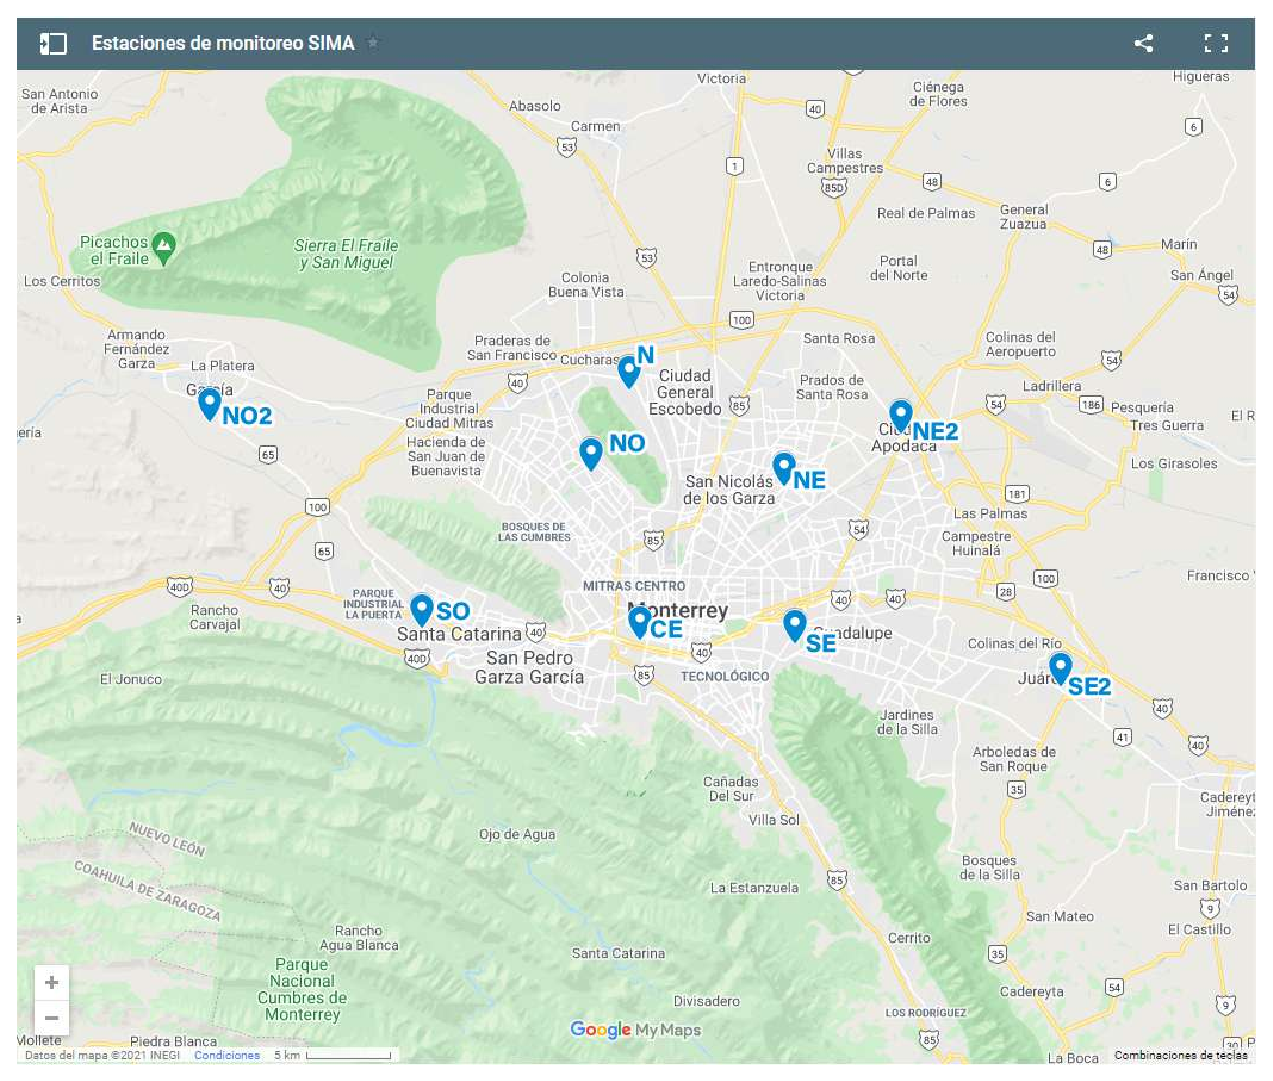
\includegraphics[trim=50 50 50 50,clip,width=1\textwidth]{mapa_estaciones.eps}
   \end{center}
    \caption{Localización de las estaciones de monitoreo de la calidad del aire.}
    \label{estaciones}
\end{figure}

\clearpage

\section{Motivación}
Existen investigaciones que ya han estudiado las relaciones entre contaminantes del aire y salud pública, sin embargo, con el presente trabajo se busca aportar a la creación de nuevas herramientas que permitan observar y estudiar dichas relaciones. El poder visualizar dichas relaciones puede ayudar a tomar medidas adecuadas que permitan aminorar los efectos negativos de los contaminantes del aire en la salud.

\section{Hipótesis}
Se plantea que con modelos de regresión se pueden obtener gráficos donde se pueden observar las relaciones entre el número de ingresos hospitalarios y los niveles de contaminantes del aire.

\section{Objetivos}
En esta sección se establece el objetivo general y los objetivos específicos sobre los que se orienta el presente trabajo.

\subsection{Objetivo general}
El objetivo de generar, implementar y evaluar modelos que muestran las relaciones existentes entre contaminantes del aire y salud pública tiene la finalidad de apoyar a la implementación de estrategias que aminoran los efectos negativos de los contaminantes del aire en la salud de las personas. Con los modelos generados se puede tener una herramienta que permite identificar gráficamente las relaciones con solo proporcionarle el conjunto de datos.

\subsection{Objetivos específicos}
\begin{itemize}
\item Generar, implementar y evaluar modelos de regresión que permite cuantificar las relaciones entre contaminantes del aire y salud pública a partir de un conjunto de datos.
\end{itemize}
\begin{itemize}
\item Diseñar e implementar visualizaciones interactivas que permiten explorar los modelos implementados y su validez estadística.
\end{itemize}
\begin{itemize}
\item Evaluar la eficacia de los modelos generados para que así al utilizar cualquiera de los modelos generados se pueda tener noción de la fiabilidad del análisis realizado a partir de los resultados producidos por los modelos.
\end{itemize}
%\begin{itemize}
%\item Generar un modelo de regresión que permite estudiar las relaciones entre los niveles de contaminantes del aire y salud pública.
%\end{itemize}

%\section{Estructura}
%El contenido de la investigación se divide en...


\chapter{Antecedentes}
%En algunos trabajos se han utilizado modelos de series de tiempo y ...
Existen factores ambientales que afectan la salud de una comunidad como: el abastecimiento de agua potable y el saneamiento, la vivienda y el hábitat, la alimentación, la contaminación ambiental, el empleo de productos químicos y los riesgos ocupacionales \citep{r2}. 

Contaminación del aire es un término usado para describir la presencia de uno o más contaminantes en la atmósfera, cuyas cantidades y características pueden resultar perjudiciales o interferir con la salud, el bienestar u otros procesos ambientales naturales \citep{r3}.

En el presente capítulo se presentan los fundamentos y definiciones de los conceptos más relevantes para el tema de estudio abordado.
%\section{Antecedentes históricos}

\section{Monitoreo de calidad del aire}
Existen diversos estudios que muestran que existen potenciales efectos a la salud cuando en el aire están presentes contaminantes en forma de partículas, gases o agentes biológicos.
%En los últimos años ha habido un desarrollo considerable de la tecnología para el control de la calidad del aire, esto como resultado de una mayor conciencia, tanto de parte de los gobiernos como de los ciudadanos, sobre la importancia de mantener el aire lo más apto posible para la vida humana.

\citet{r4} mencionan que desde inicios de 1950 se observa una preocupación por los contaminantes del aire  en los países de América Latina y el Caribe. Las universidades y dependencias de los ministerios de salud fueron los organismos que realizaron las primeras mediciones de contaminación en el aire.

En 1965, el Consejo Directivo de la Organización Panamericana de la Salud (OPS) recomendó el establecer programas de investigación de la contaminación del agua y del aire, con el objetivo de colaborar en el desarrollo de políticas adecuadas de control \citep{r5}.

Mediante el Centro Panamericano de Ingeniería Sanitaria y Ciencias del Ambiente (CEPIS), la OPS acordó establecer una red de estaciones de muestreo de la contaminación del aire.
En junio de 1967 La Red Panamericana de Muestreo Normalizado de la Contaminación del Aire (REDPANAIRE) inició sus operaciones recolectando muestras mensuales de polvo sedimentable (PS) y muestras diarias de partículas totales en suspensión (PTS) y de SO2. La REDPANAIRE comenzó con ocho estaciones y a fines de 1973 tenía un total de 88 estaciones distribuidas en 26 ciudades de 14 países \citep{r5}.

Para diciembre de 1973 se habían recolectado más de 350,000 datos sobre la calidad del aire, en los que se observa que algunas ciudades mostraban una tendencia al incremento de los niveles de contaminación \citep{r5}.

En 1980 la REDPANAIRE desapareció y pasó a formar parte del Programa Global de Monitoreo de la Calidad del Aire, iniciado en 1976 por la OMS y el Programa de las Naciones Unidas para el Medio Ambiente (PNUMA), como parte de un sistema global de monitoreo ambiental llamado GEMS por sus siglas en inglés \emph{Global Environmental Monitoring System}.

En la década de 1990, la OMS organizó, con carácter global, el Sistema de Información para el Control de la Calidad del Aire llamado AMIS por sus siglas en inglés \emph{Air Management Information System}. Entre las actividades más destacadas de AMIS se incluye el coordinar las bases de datos sobre temas relacionados con la calidad del aire.

En Nuevo León, México, las operaciones de la Red Automática de Monitoreo Atmosférico iniciaron en 1993. Dicha red en sus inicios contaba con cinco estaciones fijas de monitoreo continuo de monóxido de carbono (CO), dióxido de azufre (SO2), óxidos de nitrógeno (NOx), ozono y PM10 \citep{r4}. Como se muestra en la figura \ref{estaciones}, actualmente se cuenta con nueve estaciones fijas.

\section{Series de tiempo}
\citet{r4} mencionan que las relaciones entre niveles de concentraciones de contaminantes del aire y los efectos sobre la salud generalmente son obtenidas de estudios epidemiológicos de series de tiempo. Uno de los diseños epidemiológicos más utilizados son los estudios de series temporales. Con esos diseños se analizan las variaciones en el tiempo de la exposición al contaminante y el indicador de salud estudiado en una población \citep{r1}.

Las series de tiempo se pueden definir como un conjunto de observaciones {{ot}} tomadas en un tiempo \emph{t} determinado. Los estudios de series de tiempo relacionan estadísticamente los cambios temporales en la repercusión de cambios en la concentración de un contaminante en la población \citep{r8}.

Para mostrar datos en una serie de tiempo, especialmente en el área médica, estos suelen agruparse en \emph{semanas epidemiológicas}\footnote{Una semana epidemiológica es un estándar de medición temporal que se utiliza para comparar datos en ventanas de tiempo definidas. La primera semana epidemiológica del año termina el primer sábado de enero de cada año \citep{r7}.}. 

\section{Clasificación de enfermedades}
Existe un instrumento estadíıstico y sanitario para identificar enfermedades llamado Clasificación Internacional de Enfermedades (CIE), cuya finalidad es entender las causas de morbilidad y mortalidad de la población y así mejorar la calidad de vida de la misma. Es en base a un criterio epidemiológico y sanitario establecido por Farr a finales del siglo XIX que esta clasificación agrupa enfermedades en epidémicas, generales, locales ordenadas por origen geográfico, trastornos del desarrollo y lesiones \citep{r9}. Para lograr distinguirlas se emplea un código alfanumérico que consiste de una letra en la primera posición, seguida de dos dígitos, un punto decimal y un último dígito. El rango de valores va de A00.0 a Z99.9.

\section{Modelos de regresión lineal}
La tendencia \emph{$w_0$} de una serie de tiempo puede ser obtenida a partir de una regresión lineal de la misma \citep{r10}. Una regresión lineal es una metodología inferencial supervisada que busca predecir valores \emph{y} dado un vector de variables de entrada \emph{t} por medio del ajuste de coeficientes \emph{w} de la función lineal 
\begin{equation}
    \hat{y}(t,w) = w_0 + w_1x_1 + ... + w_tx_t.
    \label{eq1}
\end{equation}

\subsection{Regresión múltiple}
Un modelo de regresión múltiple es un modelo complemento de la regresión lineal simple, el cual tiene dos o más variables independientes \emph{k} que pueden influir en una variable dependiente \emph{y}. \citet{r11} expresan la regresión múltiple mediante la siguiente ecuación:
\begin{equation}
    y = \beta_0 + \beta_1x_1 + ... + \beta_kx_k + \varepsilon.
    \label{eq2}
\end{equation}

\section{Modelos ARIMA}
Los modelos autorregresivos integrados de media móvil o ARIMA, por su abreviatura en inglés abarcan un catalogo de aproximaciones para el estudio de series de tiempo. 

Los modelos ARIMA utilizan variaciones y regresiones de datos estadísticos con el fin de encontrar patrones para una predicción hacia el futuro. 

\chapter{Estado del arte}
En el presente capítulo se estudia literatura reciente relacionada con el presente trabajo, esto con el objetivo de revisar distintos métodos para resolver el problema planteado en el presente trabajo y, además, también revisar implementaciones similares para resolver problemas distintos. Lo anterior tiene la finalidad de comparar los trabajos revisados e identificar áreas de oportunidad en ellos.

En la primera sección, \emph{trabajos relacionados}, se recopilan obras con características relacionadas al presente trabajo, ya sean relacionados con el problema que se pretende resolver o con los métodos empleados para buscar su resolución.

En la segunda sección, \emph{análisis comparativo}, se comparan las distintas características de los trabajos revisados, de esa forma se pueden determinar las principales ventajas y desventajas de cada trabajo. 

Finalmente, en la tercera sección, \emph{áreas de oportunidad}, se realiza una conclusión acerca de los resultados obtenidos del análisis comparativo.

\clearpage
\section{Trabajos relacionados}
Se recopila literatura relacionada desde el año 2017 hasta el año 2021. En esta sección los trabajos se mencionan en orden cronológico tomando en cuenta su año de publicación.

\citet{r12} estudian la relación entre los niveles de contaminantes ambientales y la presencia de casos de enfermedades respiratorias en las consultas pediátricas. La variable dependiente analizada es la demanda en las consultas pediátricas por bronquiolitis, episodios de broncoespasmo y procesos respiratorios de vías altas. Como variables independientes se tienen los valores de contaminación ambiental. Se calculan coeficientes de correlación y regresión lineal múltiple.

\citet{r13} abordan la necesidad de monitoreo, control y predicción de la pendiente de los niveles de contaminantes del aire. Para abordar el problema de investigación utilizan modelos ARIMA. 

\citet{r14} estudian la asociación entre la exposición a largo plazo a la contaminación del aire y la metilación del ADN. Para ello realizan un estudio utilizando modelos de regresión lineal robustos para analizar la asociación entre la exposición al NO2 y a las partículas PM10 y PM2.5.

\citet{r15} en su estudio abordan los niveles de contaminación del aire y su asociación con la presencia de presión sanguínea elevada en niños y adolescentes. La exposición a partículas PM10 y PM2.5 son estimadas con un modelo espacio-temporal. Son utilizados modelos lineales de efectos mixtos y modelos de regresión logística para investigar la asociación entre la exposición a partículas PM y presión sanguínea e hipertensión. 

\citet{r16} estudian la relación entre los niveles de contaminación del aire y la obesidad y problemas cardiometabolicos. Para dicho estudio emplean modelos de regresión lineal.

\citet{r17} examinan las asociaciones entre la exposición temprana a la contaminación del aire y la incidencia de asma y rinitis alérgica desde el nacimiento hasta la adolescencia. Para su estudio utilizan modelos de regresión.

\citet{r18} estudian la asociación entre la exposición temprana a los contaminantes del aire y los egresos hospitalarios por asma. Para su estudio aplican modelos de regresión logística para el análisis de datos. 

\citet{r19} abordan el estudio de la relación entre los niveles de contaminación del aire y el número de admisiones hospitalarias. Para ello se construye un modelo basado en la distribución de Poisson.

\citet{r20} estudian la relación entre la mortalidad del coronavirus (COVID-19) y la contaminación del aire. Para dicho estudio emplean un modelo de regresión lineal para establecer la relación entre los parámetros de la contaminación del aire (concentraciones de PM10 o PM2.5) y la variable de respuesta (porcentaje
mortalidad por unidad de casos reportados).
\clearpage

\section{Comparación de trabajos}
La mayoría de los trabajos encontrados emplean modelos de regresión lineal o modelos de predicción. Además, en todos los trabajos encontrados el problema tratado presenta una alta relación con el problema abordado en el presente trabajo de tesis. El análisis comparativo de los trabajos relacionados se hace en base de los siguientes puntos:

\begin{description}
\item[Modelos de regresión lineal:]{Son aquellos que ayudan a estudiar la relación entre una variable dependiente y una o más variables independientes.}
\end{description}

\begin{description}
\item[Modelos de predicción:]{Son aquellos que ayudan a hacer predicciones de una variable.}
\end{description}

\begin{description}
\item[Evaluación de modelos:]{Se refiere a la utilización de técnicas para evaluar la eficacia de los modelos generados.}
\end{description}

\begin{description}
\item[Estudio de contaminantes del aire:]{Se refiere a que el tema de estudio incluya uno o más contaminantes del aire.}
\end{description}

\begin{description}
\item[Estudio de problemas de salud:]{Se refiere a que el tema de estudio incluya uno o más problemas de salud.}
\end{description}

En el cuadro \ref{tab:Comparación de trabajos frente al desarrollado} se desglosan que características presentes  que se pueden encontrar en las investigaciones citadas y su relación con la investigación con la que se está trabajando actualmente.\\
\renewcommand{\tablename}{Cuadro}
\renewcommand{\arraystretch}{1.4}
\begin{table}[hbt!]
\centering
\caption{Comparación de trabajos frente al desarrollado, donde $\checkmark$ indica que cumple con esta característica y  $\times$ no cumple con esta característica.}
\vspace{0.5cm}
\begin{adjustbox}{width=0.5\textwidth}
\begin{tabular}{|l|c|c|c|c|c|}
\hline
Trabajo & \rotatebox[origin=c]{90}{ Modelos de regresión lineal } & \rotatebox[origin=c]{90}{ Modelos de predicción } & \rotatebox[origin=c]{90}{ Evaluación de modelos } & \rotatebox[origin=c]{90}{ Estudio de contaminantes del aire } & \rotatebox[origin=c]{90}{ Estudio de problemas de salud }\\
	\hline
    \citet{r12} & \checkmark & $\times$ & $\times$ & \checkmark & \checkmark\\
    \hline
    \citet{r13} &  $\times$ & \checkmark & \checkmark & \checkmark & $\times$\\
    \hline
    \citet{r14} & \checkmark & \checkmark & $\times$ & \checkmark & \checkmark\\
    \hline
    \citet{r15} & \checkmark & \checkmark & $\times$ & \checkmark & \checkmark\\
	\hline    
    \citet{r16}& \checkmark & $\times$ & $\times$ & \checkmark & \checkmark\\
	\hline    
    \citet{r17} & $\times$ & \checkmark & \checkmark & \checkmark & \checkmark\\
	\hline    
    \citet{r18} & $\times$  & $\times$ & $\times$ & \checkmark & \checkmark\\
	\hline    
    \citet{r19} & \checkmark & \checkmark & $\times$ & \checkmark & \checkmark\\
	\hline    
    \citet{r20} &  \checkmark & \checkmark & $\times$ & \checkmark & \checkmark\\
	\hline    
    El presente trabajo & \checkmark & \checkmark & \checkmark & \checkmark & \checkmark\\
    \hline
\end{tabular}
\end{adjustbox}
\label{tab:Comparación de trabajos frente al desarrollado}
\end{table}
\clearpage

\subsection{Áreas de oportunidad}
Como se puede observar en el cuadro \ref{tab:Comparación de trabajos frente al desarrollado}, la mayoría de los trabajos encontrados abordan el estudio de los contaminantes del aire y salud con excepción de \citet{r13} que se enfocan en la predicción de niveles de contaminantes del aire, lo cual puede indicar que la relación entre los contaminantes del aire y salud es un tema de relevancia en la actualidad. 

Ya que la mayoría de los trabajos encontrados estudian la relación entre contaminantes del aire y salud, la mayoría de los trabajos emplean modelos de regresión lineal por que es una buena opción para el estudio de relaciones entre variables. Las excepciones, además de la ya anteriormente mencionada, son \citet{r17} y \citet{r18} quienes emplean otros tipos de modelos de regresión.

En el presente trabajo se elaboran modelos de predicción para el tratamiento de los datos empleados para los experimentos, ya que como menciona \citet{r15}, una de las limitaciones en este tipo de estudios es los campos sin llenar en los registros de datos.

En el presente trabajo también se emplean técnicas para evaluar los modelos generados. Solo en tres de los trabajos encontrados se aborda la evaluación de los modelos empleados, y al ser incluida en el presente estudio, puede representar una distinción.

\chapter{Diseño de la solución propuesta}
En el presente capítulo se presenta la propuesta de diseño de la solución para el problema de investigación abordado en el presente trabajo, así como su implementación.
%Habiendo conocido las características que mejor describen a los atributos del presente trabajo, se puede decir que la base del método propuesto se puede desarrollar.

\section{Herramientas}
Las herramientas utilizadas en la presente investigación son:
\begin{itemize}
	\item \texttt{Python 3.8.8} \url{https://www.python.org/}: Es un lenguaje de programación de alto nivel para programación de propósito general que cuenta con un conjunto de librerías de código abierto para estadísticas, limpieza y manipulación de datos.
	\item \texttt{Numpy 1.20.1} \url{http://www.numpy.org/}: Es una librería para Python que brinda soporte para arreglos y matrices grandes y multidimensionales, así como funciones matemáticas de alto nivel para operar en tales estructuras.  
	\item \texttt{Pandas 1.2.4} \url{https://pandas.pydata.org/}: Es una librería para Python diseñada para la manipulación y análisis de datos.
	\item \texttt{Seaborn 0.11.1} \url{https://seaborn.pydata.org/}: Es una librería para Python que provee una interfaz de alto nivel para la visualización de gráficos estadísticos.
	\item \texttt{Matplotlib 3.3.4} \url{https://matplotlib.org/}: Es una librería para Python que permite generar visualizaciones estáticas, animadas e interactivas a partir de datos.
	\item \texttt{Statsmodels 0.12.2} \url{https://www.statsmodels.org/}: Es una librería para Python que tiene el objetivo de que el usuario pueda explorar datos, estimar modelos estadísticos y realizar pruebas estadísticas.
\end{itemize}

\section{Metodología}

\subsection{Recolección de datos}
La primera fase es la recolección de datos. El objetivo es tener un archivo que contenga datos de los niveles de uno o más  contaminantes del aire en años recientes y también del mismo lugar tener datos del número de egresos hospitalarios durante esos años. Los datos de egresos hospitalarios provienen de la base de datos de la Secretaría de Salud del Gobierno de México \cite{f1}. También se tienen registros de los niveles de algunos contaminantes del aire presentes en el área metropolitana de Monterrey, dichos registros son hechos por las estaciones de monitoreo pertenecientes al SIMA \cite{f2} mostradas en la figura \ref{estaciones}. Los documentos con los datos son proporcionados por \citeauthor{f3}.
% TABLA CIES

\subsection{Selección y agrupación de datos}
Después de la recolección de datos se procede a seleccionar que datos van a ser utilizados para los experimentos. Para ello se utiliza Python con la librería Pandas que permite la manipulación de datos. Los conjuntos de datos por años de egresos hospitalarios contienen información de todos los estados de México, por lo cual se tendría que hacer una limpieza de datos para solo obtener los registros de Nuevo León.

Para la selección y agrupación de datos se sigue el procedimiento mostrado en la figura \ref{alg:a1}.

\begin{algorithm}
\caption{An algorithm with caption}\label{alg:a1}
\begin{algorithmic}[1]
\State $a \leftarrow $ años de los que se obtuvieron datos
\For {$i \in a$}
    \State $contaminantes \leftarrow $ nombre del archivo .csv que contiene los datos de los contaminantes en el año $i$
    \State Leer en $contaminantes$ las columnas fecha y contaminante 
    \State $egresos \leftarrow $ nombre del archivo .csv que contiene los datos de los contaminantes en el año $i$
    \State Leer en $contaminantes$ las columnas fecha, padecimiento y estado
    \State $estado \leftarrow $ estado del que se quieren obtener datos
    \State Seleccionar en $contaminantes$ los datos del $estado$
\EndFor
\end{algorithmic} 
\end{algorithm}

\subsection{Visualización de la evolución de las variables}
Al ya tener seleccionados los datos a utilizar se procede a elaborar gráficos en Python que muestran la evolución de las variables en el tiempo. Para ello se generan los tipos de gráficos discutidos a continuación.

\subsubsection{Series de tiempo}
Se realizan series de tiempo en Python (citar) con ayuda de la librería matplotlib, sklearn y seaborn, ya que son herramientas accesibles que ayudan a la generación de este tipo de gráficos. 
En la figura \ref{serie_de_tiempo} se muestra un ejemplo de las series de tiempo generadas.
\begin{figure}[h!]
\setcounter{figure}{0} % por culpa de sciposter
\captionsetup{type=figure} % por culpa de sciposter
\begin{center}
   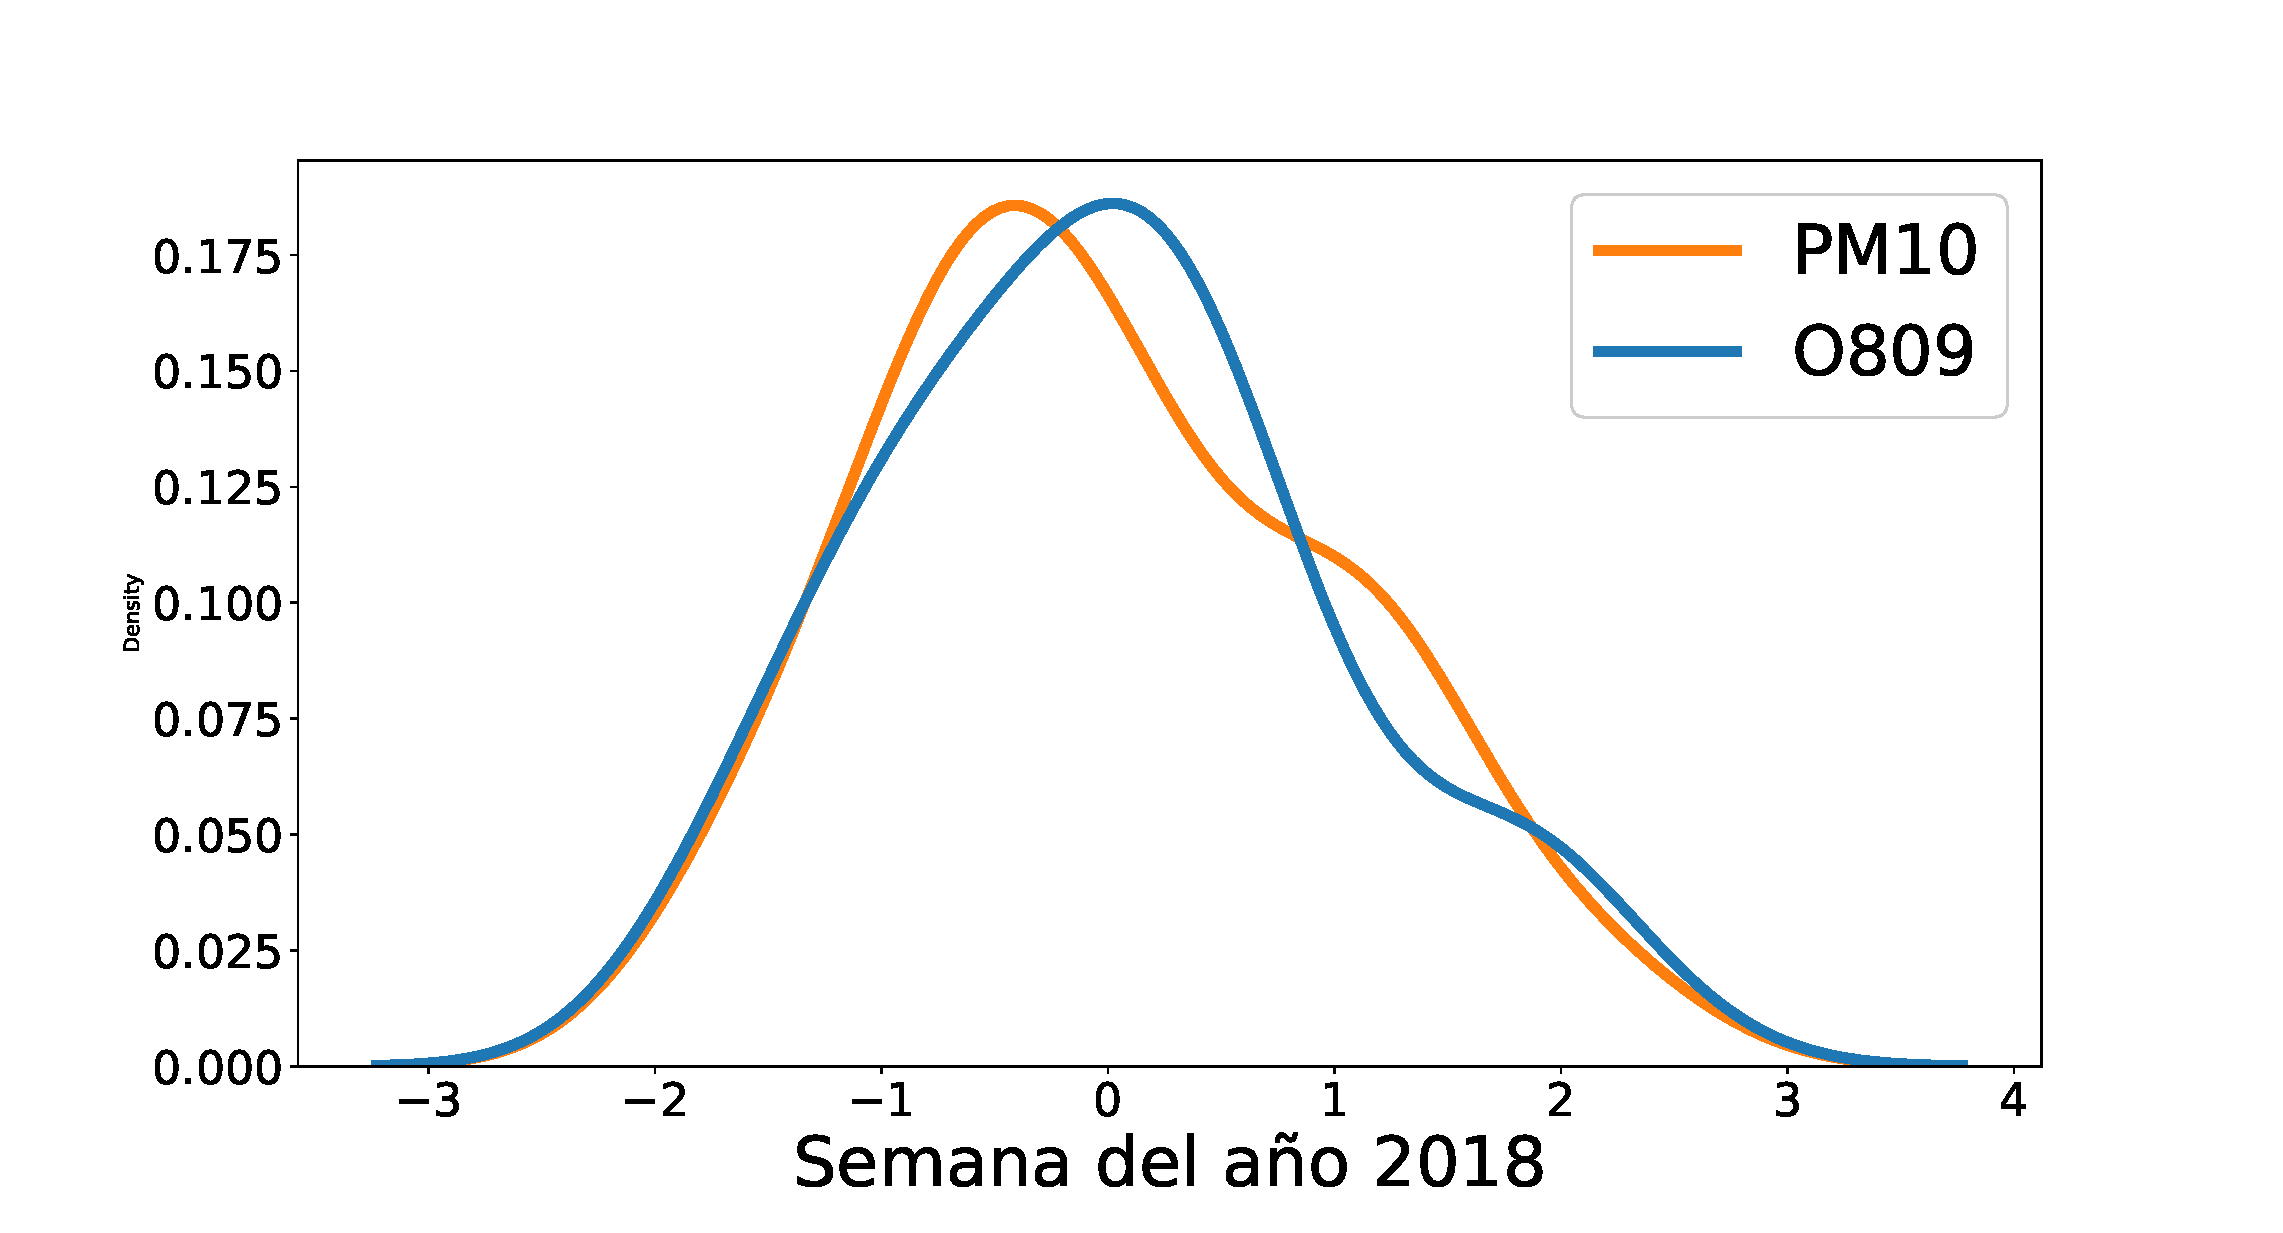
\includegraphics[width=1.1\textwidth]{PM10_O809_2018.eps}
   \end{center}
    \caption{Evolución de los niveles de PM10 y el número de egresos diagnosticados la CIE O809 en el 2018.}
    \label{serie_de_tiempo}
\end{figure}

\subsubsection{Gráficos de radar}
Los gráficos de radar o diagramas de telaraña son otra manera de visualizar un conjunto de datos. Sirven para comparar variables visualizando si existen valores o patrones de evolución en el tiempo similares entre ellas. Es por ello que en el presente trabajo se elaboran gráficos de radar con ayuda de Python y las librerías numpy y matplotlib. En la figura \ref{grafico_de_telaraña} se muestra un ejemplo de los gráficos de telaraña generados.
\begin{figure}[h!]
\setcounter{figure}{1} % por culpa de sciposter
\captionsetup{type=figure} % por culpa de sciposter
\begin{center}
   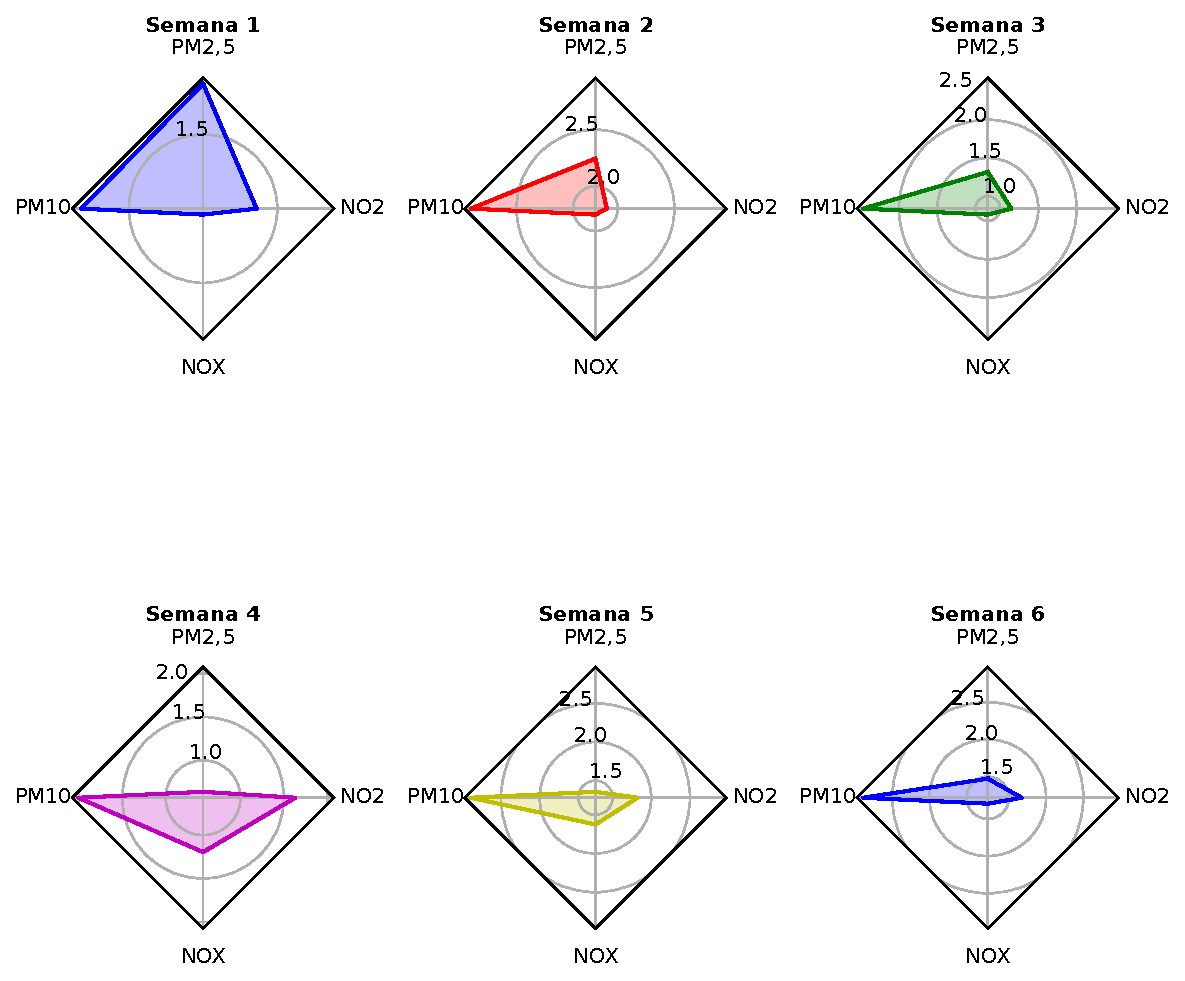
\includegraphics[width=1\textwidth]{Contaminantes-2017.eps}
   \end{center}
    \caption{Niveles de los contaminantes NO2, NOX, PM10, y PM2.5 durante las primeras 6 semanas del 2017.}
    \label{grafico_de_telaraña}
\end{figure}
\clearpage

\subsection{Implementación de modelos para el estudio de la relación entre las variables}
Después de haber generado gráficos para la visualización de la evolución de las variables, se procede a generar modelos para el estudio de la relación entre las variables. Para ello se utiliza Python y la librería statsmodels. Los tipos de modelos generados son los siguientes:
\begin{itemize}
	\item Regresión lineal.
	\item Regresión lineal múltiple.
	\item ARIMA.
\end{itemize}

\chapter{Implementación de la solución propuesta}
Recapitulando las fases anteriores, se conoce que...


\chapter{Experimentos}
Después de...

\section{Diseño experimental}
Hola...

\section{Resultados}
Establecidos los experimentos que se van a realizar, se reporta los resultados obtenidos...

\section{Discusión}
Todos los experimentos son ejecutados en una laptop con las especificaciones del cuadro \ref{tab:Especificaciones técnicas del PC}.

\begin{table}[H]
	{\centering
		\caption{Especificaciones técnicas del equipo de cómputo}
		\begin{tabular}{|c|c|c|}
			\hline
			Sistema Operativo & Windows 10 64 bits\\
			\hline
			Procesador & Intel Core i5-7300HQ\\
			\hline
			RAM & 8 GB RAM DDR4 2133 MHz\\
			\hline
		\end{tabular}

	\label{tab:Especificaciones técnicas del PC}
	}
\end{table}


\chapter{Conclusiones}
Este capítulo describe la tesis a partir de la manera que cumple los objetivos generales y específicos para determinar si la hipótesis se comprueba, trata también del porque se realizó la tesis...

\clearpage

\section{Contribuciones}
La solución propuesta surgió a partir de...

\section{Trabajo a futuro}
La solución propuesta en la tesis...